\section{Extended Position Based Dynamics} \label{ch2:xpbd} %название по-русски
	В статье \cite{muller2020detailed} авторами оригинальной статьи Position Based Dynamics были обозначены шесть основных проблем данного алгоритма
	\begin{enumerate}[1.]
		\item Он не использует физические параметры и размерности
		\item Жесткость зависит как от итерации, так и от размера временного шага
		\item Интеграция не является физически точной
		\item Он зависит от порядка обхода ограничений
		\item Он зависит от структуры геометрии
		\item Он медленно сходится
	\end{enumerate}
	Для решения первых трех, авторами был разработан алгоритм Extended Position Based Dynamics \cite{xpbd}. Для этого, авторы взяли известное уравнение
	\begin{equation}
		\textbf{M}\ddot{x} = -\nabla U^T(x)
	\end{equation}
	В данном уравнении, под $M$ понимаются массы частиц, под $x$ их положения, а в под $U$ - потенциальная энергия. Если дискретизировать данное уравнение по времени, то мы получим следующее уравнение
	\begin{equation}
		\textbf{M}(\frac{x^{n+1} - 2x^n + x^{n-1}}{\delta t^2}) = -\nabla U^T(x^{n+1})
	\end{equation}
	
	Записав потенциальную энергию через функции ограничения описанных в \cite{servin2006interactive}, мы получаем систему уравнений
	\begin{equation} \label{eq:xpbd_first}
		\textbf{M}(x^{n+1} - 2x^n + x^{n-1}) - \nabla \textbf{C}(x^{n+1})^T\lambda^{n+1} = 0
	\end{equation}
	\begin{equation} \label{eq:xpbd_second}
		\textbf{C}(x^{n+1}) + \frac{\alpha}{\delta t^2}\lambda^{n+1} = 0		
	\end{equation}
	
	В данной системе $\textbf{C} = [C_1(x), C_2(x),... C_M(x)]^T$ - вектор состоящий из функций ограничения, $\lambda = [\lambda_1, \lambda_2, ..., \lambda_M]^T$ - вектор множителей ограничений, $alpha$ - диагональная матрица содержащая обратную жетскость каждого ограничения. Если мы обозначим выражение в \ref{eq:xpbd_first} как $g(x, \lambda) = 0$, а выражение \ref{eq:xpbd_second} как $h(x, \lambda) = 0$, то воспользовавшись методом Ньютона для решения полученных систем, мы получаем систему вида:

\begin{equation} \label{eq:xpbd-system-hard}
	\left[
		\begin{array}{cc}
			\frac{\delta g}{\delta x} & -\nabla \textbf{C}^T(x_i)\\
			\nabla \textbf{C}(x_i) & \frac{\alpha}{\delta t^2}
		\end{array}
	\right]\left[
		\begin{array} {c}
			\delta x\\
			\delta \lambda
		\end{array}
	\right]	= -\left[
		\begin{array}{c}
			g(x_i, \lambda_i)\\
			h(x_i, \lambda_i)
		\end{array}
	\right]
\end{equation}
	Далее, авторы статьи вносят две аппроксимации. Первая - принимается что $\frac{\delta g}{\delta x} = M$. Это исключает геометрическую жесткость и вносит погрешность порядка $O(\delta t^2)$ (данный метод тогда можно рассматривать как квази-Ньютоновский). Вторая - $g(x_i, \lambda_i) = 0$. Хотя это верно только для первой итерации метода Ньютона (при $x_0 = 2x^n + x^{n-1}, \lambda_0 = 0$), если $\nabla \textbf{C}^T$ будет изменяться медленно, то значение $g(x_i, \lambda_i)$ будет отставаться малым, и приравняется нулю, когда $\nabla \textbf{C}^T$ станет константным. Если внести эти две аппроксимации, то система \ref{eq:xpbd-system-hard} будет иметь вид 
\begin{equation} \label{eq:xbd-system-hard}
	\left[
	\begin{array}{cc}
		\textbf{M} & -\nabla \textbf{C}^T(x_i)\\
		\nabla \textbf{C}(x_i) & \frac{\alpha}{\delta t^2}
	\end{array}
	\right]\left[
	\begin{array} {c}
		\delta x\\
		\delta \lambda
	\end{array}
	\right]	= -\left[
	\begin{array}{c}
		0\\
		h(x_i, \lambda_i)
	\end{array}
	\right]
\end{equation}
	Взяв дополнение Шура мы можем получить следующую систему относительно $\delta \lambda$
\begin{equation} \label{eq:xbd-delta-lambda}
	\left[\nabla \textbf{C}(x_i) \textbf{M}^{-1} \nabla \textbf{C}^T(x_i) + \frac{\alpha}{\delta t^2}\right]\delta \lambda = -\textbf{C}(x_i) - \frac{\alpha}{\delta t^2}\lambda_i
\end{equation}	
	А значение $\delta x$ может быть высчитано используя следующее выражение.
\begin{equation} \label{eq:xbd-delta-x}
	 \delta x = \textbf{M}^{-1} \nabla \textbf{C}^T(x_i) \delta \lambda
\end{equation}	
	Заметим, что выражение \ref{eq:xbd-delta-x} совпадает с выражением \ref{eq:delta_p_pbd_2} описанным в главе \ref{ch2:pbd}, если принять $\delta \lambda$ равной $scaleFactor$. Выпишем $\delta \lambda$ в том же стиле, в котором представляется $scaleFactor$ в \ref{eq:delta_p_scaleFactor_2}.
\begin{equation} \label{eq:xbd-delta-lambda}
	\delta \lambda = \frac{-\textbf{C}(x_i) - \frac{\alpha}{\delta t^2}\lambda_i}{\nabla \textbf{C}(x_i) \textbf{M}^{-1} \nabla \textbf{C}^T(x_i) + \frac{\alpha}{\delta t^2}}
\end{equation}	
	Данное выражение отличается от представленного  \ref{eq:delta_p_scaleFactor_2} тем, что в числителе появилось слагаемое $- \frac{\alpha}{\delta t^2}\lambda_i$, а в знаменателе $\frac{\alpha}{\delta t^2}$. Именно эти два слагаемых позволяют убрать физически некорректный параметр жесткости $k$ используемый в алгоритме PBD, и использовать вместо него физически корректный параметр жесткости, используя табличные значения, получаемые из реального мира. Заметим также, что оба вышеприведенных слагаемых так-же зависят от шага времени, а значит жесткость не будет зависеть от размера временного шага. Помимо этого, на каждой итерации алгоритма используется разное значение $\lambda_i$ что также нейтрализует зависимость жесткости от количества итераций. При этом, если рассмотреть ситуацию, при которой параметр жесткости равен бесконечности, то матрица $\alpha$ будет равна нулевой, и алгоритм XPBD превращается в алгоритм PBD.
	Получившийся алгоритм XBPD представлен на \firef{alg:ExtendedPositionBasedDynamics}.
	
	\begin{algorithm} %[h]
		\SetKwFunction{algoXPBDPseudocode}{} 
		\SetKwProg{myalg}{Algorithm}{}{} %write in 2nd agrument <<Algorithm>>, <<Procedure>> etc
		\nonl\myalg{\algoXPBDPseudocode}{
			\KwInput{
				время шага симуляции $\delta t$,
				количество итераций $solverIteration$,
				текущее состояние частиц,
				предыдущее состояние частиц,
				ограничения,
				функция суммы внешних сил $f_{ext}(p)$,
			}
			\KwOutput{положение частиц спустя заданное время $p_i(t + \delta t)$}
			
			\lFor {$\forall p_i $}{
				$v_i \leftarrow \frac{p_i(t) - p_i(t -\delta t)}{\delta t} + \delta t * im_i * f_{ext}(p_i)$;
			}
			
			$dampVelocities(v_1, ... v_N)$

			\lFor {$\forall j \in 1..M $}{$\lambda_j = 0$}
			
			\For {$\forall p_i $}{
				$p^*_i \leftarrow p_i(t) + v_i * \delta t $;
				
				$generateCollisionConstraints(p_i -> p^*_i)$;
			}
						
			\For{$\forall k \in 1..solverIteration$}{
				$p^*_1, ..., p^*_N \leftarrow projectXPBDConstraints(\delta t, p^*_1, ..., p^*_N, \lambda_1, ..., \lambda_M)$;
			}
			
			\lFor {$\forall p_i $}{
				$p_i(t + \delta t) \leftarrow p^*_i$\
			}
		}
		\caption{Псевдокод алгоритма Extended Position Based Dynamics}\label{alg:ExtendedPositionBasedDynamics}
	\end{algorithm}
	\FloatBarrier
	
	Соответствующий алгоритм $solveXPBDConstraint$ представлен на \firef{alg:SolveXPBDConstraint}

	\begin{algorithm} %[h]
		\SetKwFunction{solveXPBDConstraint}{} 
		\SetKwProg{myalg}{Algorithm}{}{}
		\nonl\myalg{solveXPBDConstraint}{
			\KwInput{
				входные параметры алгоритма $solveConstraint$,
				время шага симуляции $\delta t$,
				значения $\alpha$ и $\lambda$ ограничения,
			}
			\KwOutput{необходимый сдвиг для удолветворения ограничению $\delta p^*_i$, новое значение $\lambda$}
		
			$s = \frac{\alpha}{\delta t^2}$
		
			$scaleNum = -C(p^*_1, ...) - s \lambda$
		
			$scaleDenum = \sum_{i}(im_i *|\nabla_{p^*_i} C(p^*_1, ..., p^*_{n})|^2) + s$
		
			$scaleFactor = scaleNum/scaleDenum$
		
			$\lambda = \lambda + scaleFactor$
		
			\For {$\forall p^*_i$}{
				$\delta p^*_i = scaleFactor * im_i * \nabla_{p^*_i} C(p^*_1, ..., p^*_{n})$;
			}
		}
		\caption{Псевдокод алгоритма solveXPBDConstraint}
		\label{alg:SolveXPBDConstraint}
	\end{algorithm}
	\FloatBarrier
	\newpage
	
	\begin{figure}[ht!] 
		\center
		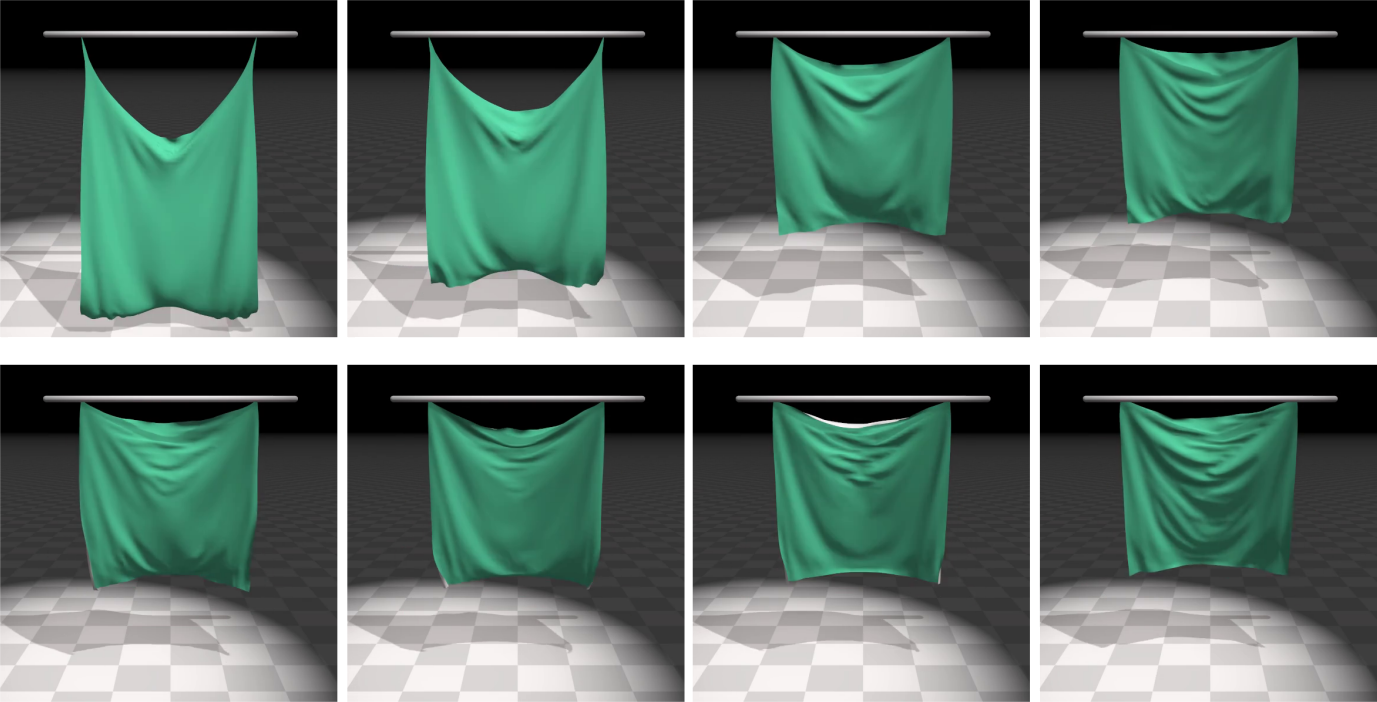
\includegraphics [scale=0.4] {my_folder/images//pbd_vs_xpbd}
		\caption{Сравнение работы алгоритма PBD и XPBD на примере свисающей ткани спустя 20, 40, 80, 160 итераций(слева направо). Верхняя строка PBD, нижняя XPBD. Можно заметить что жесткость в алгоритме PBD нелинейно зависит от числа итераций, тем временем жесткость ткани при использовании алгоритма XPBD качественно неизменна }
		\label{fig:pbd-vs-xpbd}  
	\end{figure}
	
	Единственным недостатком данного алгоритма является то, что для подсчета требуется дополнительная память для хранения параметров $\lambda$. Однако, вскоре авторами была выпущена ещё одна статья \cite{macklin2019small}, в которой ими было обнаружено, что вместо того, чтобы увеличивать количество итераций $solverIteration$, более эффективно запускать весь алгоритм $solverStep$ раз, с уменьшенным размером шага. Таким образом, ими был предложена техника Small Steps, представленная на \firef{alg:ExtendedPositionBasedDynamicsSmallSteps}. При этом крайний случай, при котором $solverIteration = 1$ не только является достаточно корректным и стабильным, но и позволяет избавится от доплнительных затрат памяти и процессорного времени на параметры $\lambda$, так как на первой итерации они равны 0.
	
		
	\begin{figure}[ht!] 
		\center
		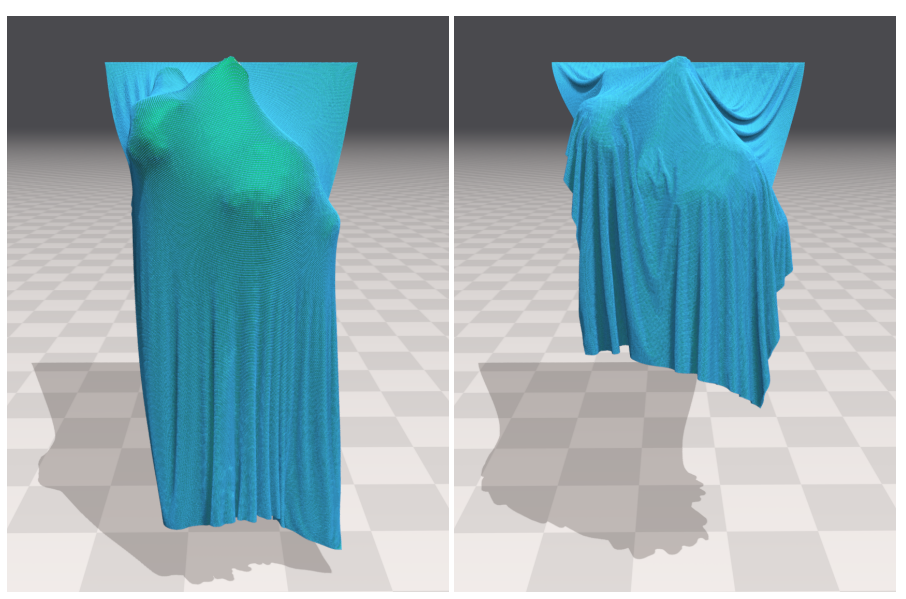
\includegraphics [scale=0.3] {my_folder/images//smallsteps}
		\caption{Сравнение XPBD вместе с техникой Small Steps. Слева $solverIteration = 30, solverStep = 1$, справа $solverIteration = 1, solverStep = 30$}.
		\label{fig:smallstep}  
	\end{figure}
	
	\begin{algorithm} %[h]
		\SetKwFunction{algoXPBDSmallStepsPseudocode}{} 
		\SetKwProg{myalg}{Algorithm}{}{} %write in 2nd agrument <<Algorithm>>, <<Procedure>> etc
		\nonl\myalg{\algoXPBDSmallStepsPseudocode}{
			\KwInput{
				время шага симуляции $\delta t$,
				количество шагов $solverStep$,
				количество итераций $solverIteration$,
				текущее состояние частиц,
				предыдущее состояние частиц,
				ограничения,
				функция суммы внешних сил $f_{ext}(p)$,
			}
			\KwOutput{положение частиц спустя заданное время $p_i(t + \delta t)$}
			
			$stepT = \delta t / solverStep$;
			
			\For{$\forall step \in 1..solverStep$}{
				\lFor {$\forall p_i $}{
					$v_i \leftarrow \frac{p_i(t + (step - 1) * stepT) - p_i(t - (step - 2) * stepT)}{stepT} + stepT * im_i * f_{ext}(p_i)$;
				}
			
				$dampVelocities(v_1, ... v_N)$
			
				\lFor {$\forall j \in 1..M $}{$\lambda_j = 0$}
			
				\For {$\forall p_i $}{
					$p^*_i \leftarrow p_i(t) + v_i * stepT $;
				
					$generateCollisionConstraints(p_i -> p^*_i)$;
				}
			
				\For{$\forall k \in 1..solverIteration$}{
					$p^*_1, ..., p^*_N \leftarrow projectXPBDConstraints(stepT, p^*_1, ..., p^*_N, \lambda_1, ..., \lambda_M)$;
				}
			
				\lFor {$\forall p_i $}{
					$p_i(t + step * stepT) \leftarrow p^*_i$\
				}
			}
		}
		\caption{Псевдокод алгоритма Extended Position Based Dynamics с использованием техники Small Steps }\label{alg:ExtendedPositionBasedDynamicsSmallSteps}
	\end{algorithm}
	\FloatBarrier

	
	
%% Вспомогательные команды - Additional commands
%
%\newpage % принудительное начало с новой страницы, использовать только в конце раздела
%\clearpage % осуществляется пакетом <<placeins>> в пределах секций
%\newpage\leavevmode\thispagestyle{empty}\newpage % 100 % начало новой страницы